\chapter[Methods of Multiresolution Modelling]{Methods for Multiresolution Modelling}
\markboth{Methods for Multiresolution Modelling}{}
\label{ch:multiresmodel}

\begin{fquote}[Douglas Merrill]With too little data, you won’t be 
able to make any conclusions that you trust.  With loads of data 
you will find relationships that aren’t real… Big data isn’t 
about bits, it’s about talent.
\fqsource{Former CIO and VP of Engineering at Google} \end{fquote} 

\begin{synopsis}
The abundance of multiresolution data and increasing benefits of
analysing multiple datasets within a single analysis have given
major impetus to the research in multiresolution data analysis. 
In application areas where division of data across different 
resolutions is smooth, wavelets~\cite{jawerth94}, multiscale 
methods~\cite{barth2002multiscale,e2011principles}, and 
scale space theory~\cite{lindeberg94} have been popularly 
used to analyse multiresolution data. This chapter discusses 
the core of the thesis and includes most of the scientific 
contributions of this thesis. This chapter also summarises 
four of the five publications contained in this thesis.
\end{synopsis}


\section{Data Transformation}
\label{s:dataTransformation}
Standard algorithms, such as mixture models, are 
unable to model multiresolution data in their 
standard form. Therefore, in~\citepub{c1}, we propose 
data transformation methods to analyse multiresolution data 
by transforming the data to different resolutions and integrating 
the data in the same resolution. 
We can then apply the algorithm on the combined data in 
a single resolution. The methodology of data transformation
integrates data in different resolutions and therefore, 
resembles fusion techniques~\cite{carter1998analysis}.


Data transformation methods, also called sampling methods, 
proposed in~\citepub{c1} are non--stochastic. 
Sampling resolution in genomics explains the level of precision 
for measuring the results of a particular experiment: either 
global (coarse resolution) or  detailed (fine resolution). As 
discussed in Section~\ref{s:multchrdata} and also shown in 
the Figure~\ref{Fig:chr21}, the relationship between different 
resolutions of chromosome, i.e., correspondence of each of the 
regions in genome in different resolutions are known  
apriori~\cite{shaffer05}. We propose two different data 
transformation methods to transform data across fine and coarse 
resolution using the knowledge of the correspondence of chromosomal 
regions in  different resolutions. 

\begin{enumerate}
\item Upsampling transforms the data from coarse resolution 
to fine resolution  increasing the dimensionality of the data.
We make multiple copies of a chromosomal region in coarser 
resolution to upsample the data in coarse resolution to fine 
resolution. 
\item Downsampling transforms the data resolution from fine 
resolution to coarse resolution  decreasing the dimensionality 
of the data. We downsample using three different methods:
OR--function, Weighted, and Majority Decision. We consider the
chromosomal amplification pattern of neighbouring chromosomal
regions if the number of  aberrated chromosomal regions and 
the number of unaberrated  chromosomal regions are equal.
\begin{enumerate}
\item In OR--function downsampling, a chromosomal region in the coarse
resolution is aberrated if any of the chromosomal regions in the fine 
resolution is aberrated.
\item Division of the regions of a chromosome are highly irregular 
and the length of a region  often differs from the 
next~\cite{shaffer05}. In weighted downsampling, a chromosomal 
region in coarse resolution is aberrated if the total length of the 
aberrated chromosomal regions is greater than total length of 
unaberrated chromosomal regions in fine resolution.
\item In majority decision downsampling, a chromosomal region in
the coarse resolution is aberrated if majority of the chromosomal
regions in the fine resolution are aberrated.
\end{enumerate}
\end{enumerate}

\subsection*{Experiments on Data Transformation}
\label{ss:DtaTransExp}

\begin{figure}[h!]
\centering
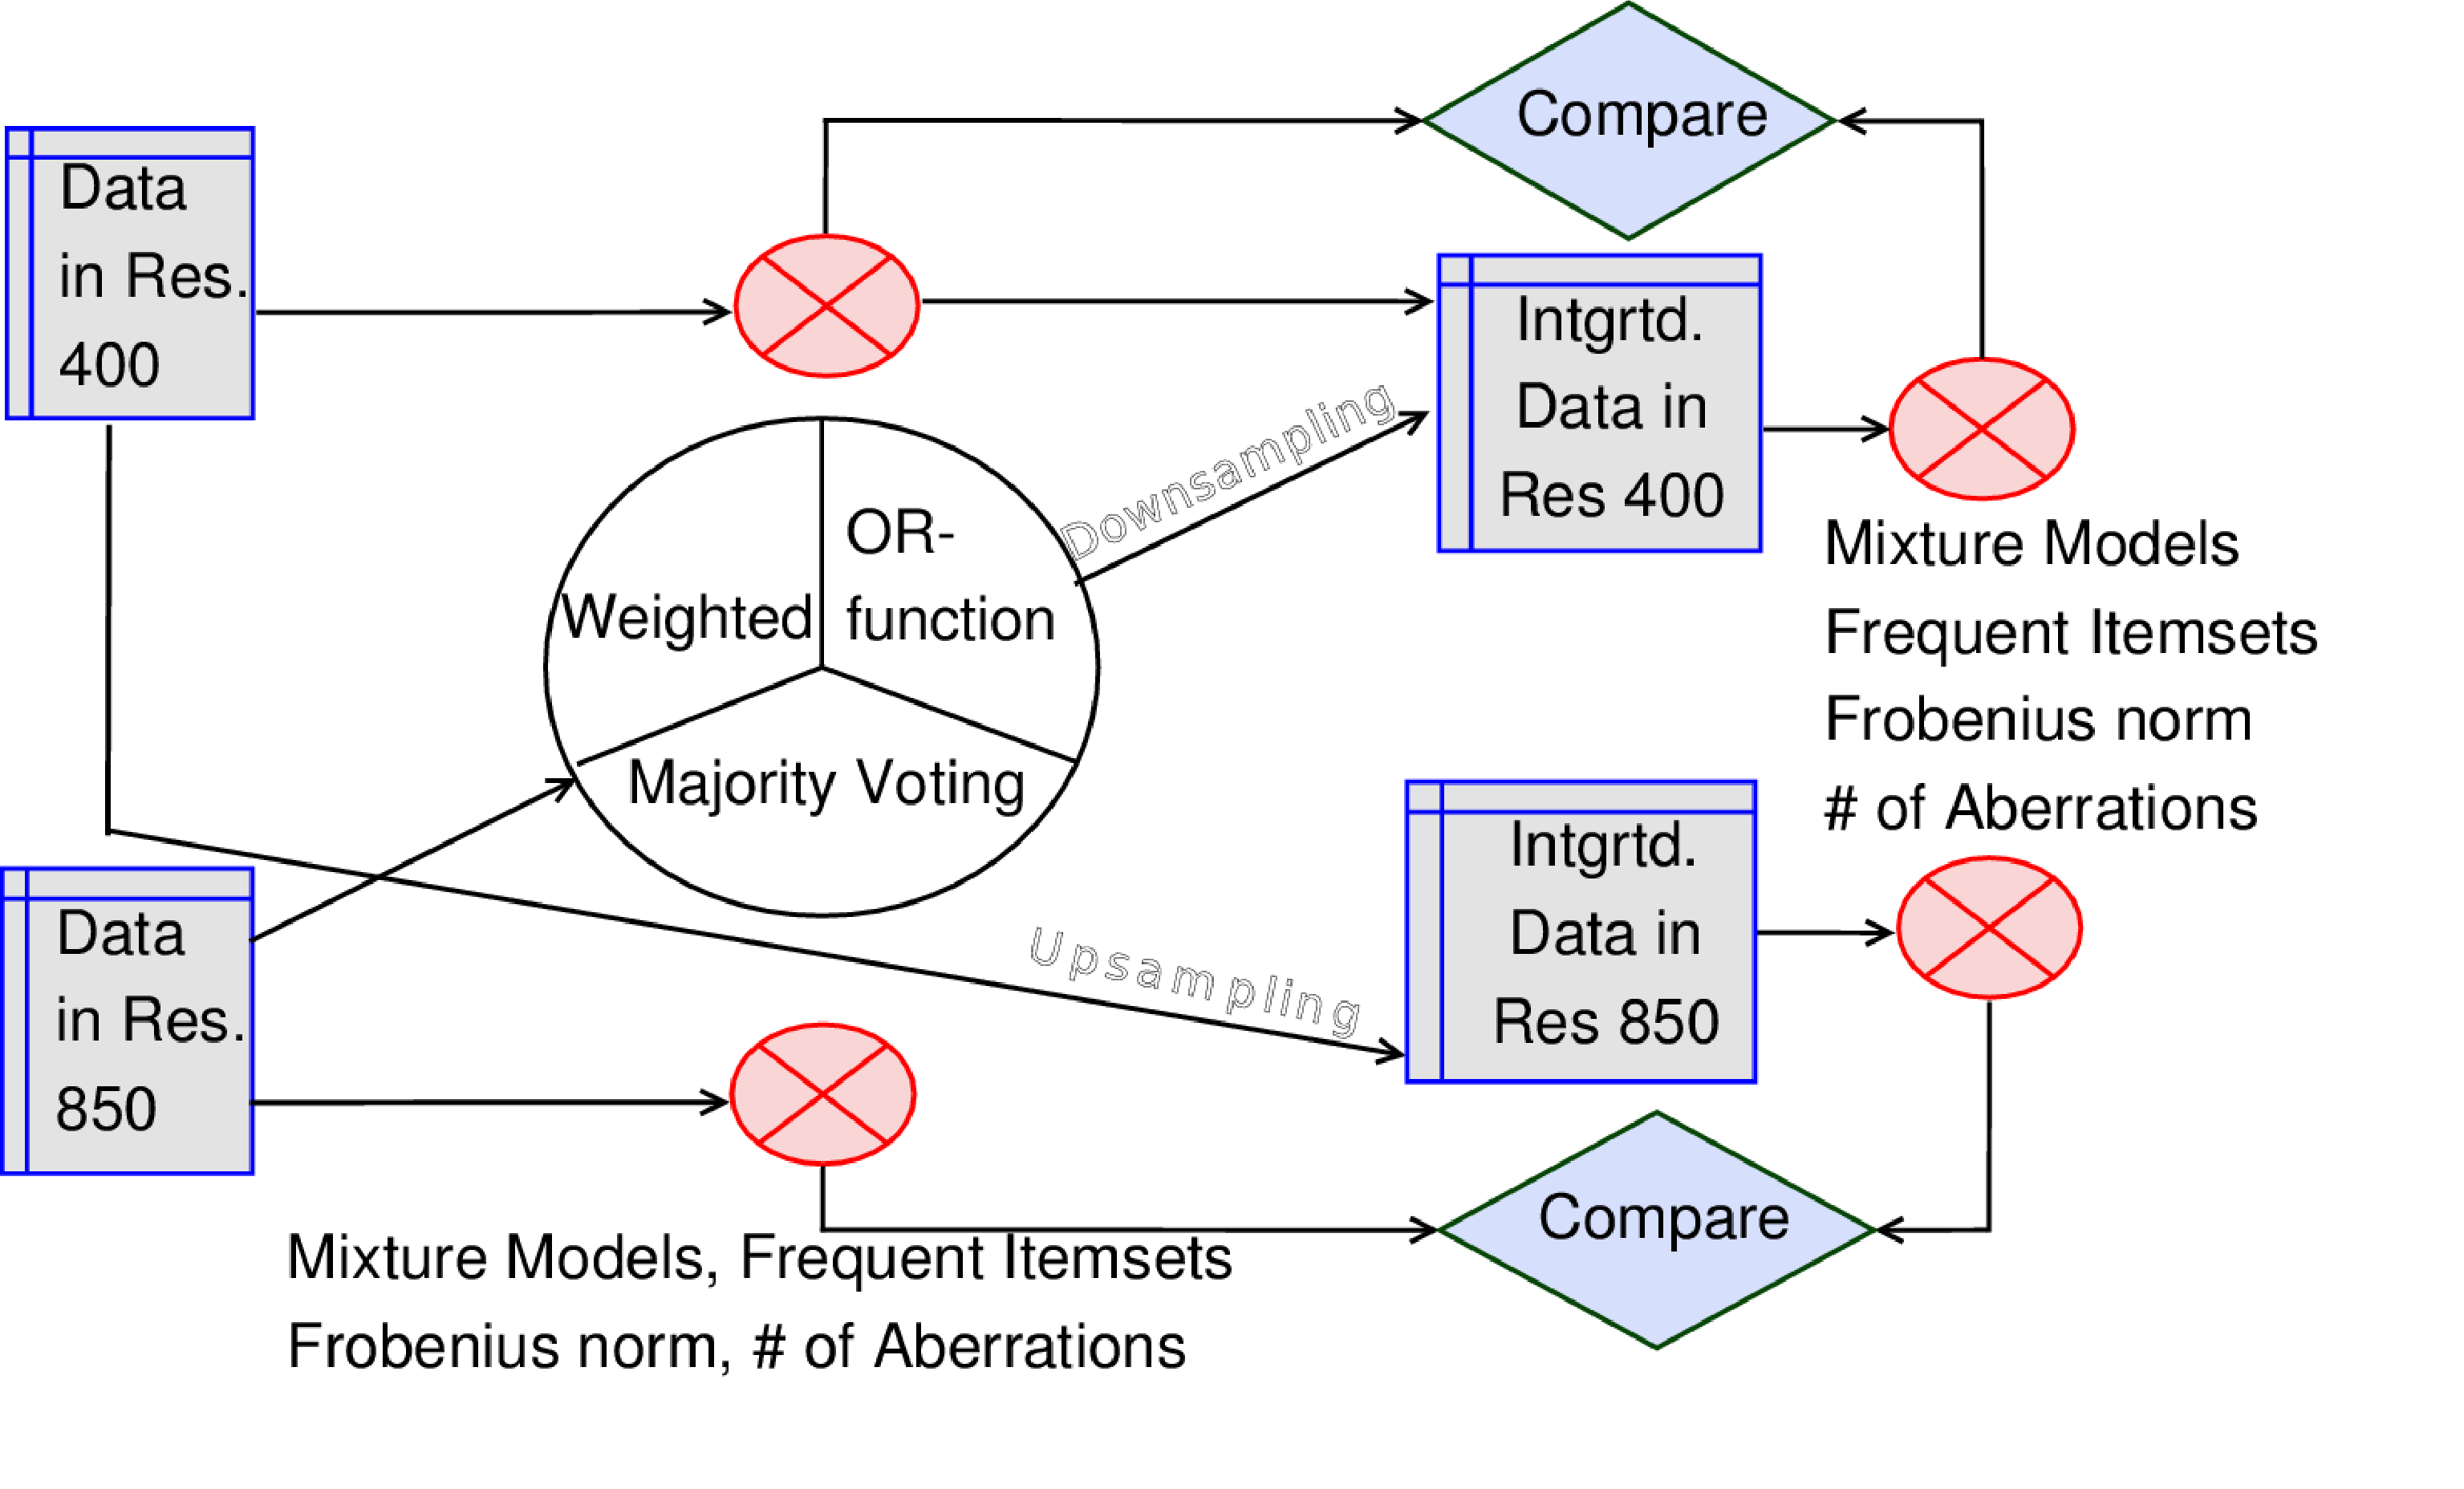
\includegraphics[trim=10mm 10mm 30mm 2mm,width=0.9\textwidth]{figures/pub1exp}
\caption[Experimental Procedure in~\citepub{c1}.]
{Schematic representation of experimental procedure of data transformation 
methods for multiresolution modelling. First, the data in two different 
resolutions are transformed to other resolutions. After transformation 
datasets in the same resolution are integrated. Finally, the algorithm
is applied on the integrated dataset. For comparative purposes the  
algorithm is also applied on the original data before data transformation.} 
\label{Fig:transexp}
\end{figure}
Figure~\ref{Fig:transexp} depicts the overall experimental procedure
where one of the three different downsampling methods transforms the 
data in fine resolution to coarse resolution. Similarly, a deterministic
upsampling method transforms the data in the coarse resolution to the 
fine resolution. Before data transformation, algorithms such as 
mixture models, and pattern mining are applied on the data in original
resolution. We then integrate the data obtained in same resolution after
data transformation. The algorithm is again applied on the  integrated 
data. Finally, we compare the results of the analysis before transformation 
and after integration in terms of the patterns obtained and model fitting.

Experiments with mixture 
modelling in different resolutions reported in~\citepub{c1} show that 
validation likelihood of the mixture  models is higher in the coarser 
resolution compared to the finer resolution. However, the model 
selection results are similar across different resolutions as 
similar number of components are selected in both the coarse and 
the fine resolution. Although similar number of components are 
selected, mixture models in coarse resolution produces better 
likelihood values than the data in fine resolution. In addition, 
time complexity is higher in the models in  the finer resolution. 
This degradation of performance in  fine resolution data can be 
attributed to the ``curse of dimensionality'' 
phenomenon~\cite{bellman61}, or Hughes effect~\cite{hughes68}. 
Models in coarse resolution  are also suitable for understanding 
and interpreting the results~\cite{Hollmen2007a}. 

The results in~\citepub{c1} also show that the mixture models 
produce better results on the combined data with the similar
number of components than the standalone data in single 
resolution. This proves the property of mixture model which 
states that number of components in the mixture model scales
with the complexity of the data not with the sample size of 
the data~\cite{hammoud2000}. The increased sample size 
arising from the integration of data from other resolution 
helps nullify the curse of dimensionality and
constrains the complexity of mixture models, and avoid 
overfitting.


MAFIA (MAximal Frequent Itemset Algorithm)~\cite{burdick01} was
used to mine maximal frequent itemsets in data in the original 
resolution and the sampled resolution to determine if the data 
transformation methods preserves the patterns in the data. The 
results in~\citepub{c1} show that data transformation across 
resolutions preserves the maximal frequent itemsets with 
negligible differences. The negligible differences are expected 
because data in coarse resolution cannot subsume all the 
information of the data in fine resolution. 

In our earlier 
research~\cite{adhikari2010b}, we have also tested the 
statistical significance  of the frequent itemsets (not the
maximal frequent itemset) to show that data transformation 
across different resolution preserves
the statistically significant patterns present in the data.
In addition, results in~\cite{adhikari2010b} also show
that statistically significant patterns are also preserved
by the generative property of mixture models in all the 
resolutions.  We also compare three different downsampling methods 
using metrics such as the Frobenius norm~\cite{stewart1998}.
Experimental results in~\citepub{c1} show that the resulting
data produced by three downsampling methods are similar 
to each other; the variation, if any are negligible.


\section{Merging of Mixture Components}
\label{s:meringMixCompo}
In~\citepub{c2}, we use merging of the mixture components of  
different mixture models in different resolutions to model the 
multiresolution data.  Mixture models can also be used in clustering 
where component distributions are used as clusters in the data.
Proposed multiresolution modelling algorithm resembles clustering
aggregation algorithm in~\cite{gionis07ca}. The similarity with 
clustering aggregation is that we use multiple clustering results,
i.e., mixture models to improve the mixture modelling. However, 
clustering aggregation clusters single dataset generating results
as a single clustering solution. In contrast, the proposed multiresolution
modelling algorithm analyses different datasets in different 
resolutions generating clustering solutions in 
different resolutions. 

In the proposed multiresolution modelling 
algorithm, we first apply mixture models on the data in each 
resolution separately. Secondly, we 
iteratively merge the similar mixture components in different 
mixture models in different resolutions. This is unlike~\citepub{j1}
where we merge the components from the same mixture model. We 
extend the derivation of fast approximation of Kullback Leibler
divergence as a criterion in~\citepub{j1} to determine the  
similarity between the mixture components to two mixture 
models as:

\begin{eqnarray}
\label{eq:symmcfmulti}
KL & = & \displaystyle \sum_{i \in X^{*}} \pi_{\alpha} \displaystyle
\prod _{m=1}^{{d}}
\left(\alpha_m^{X^{*}_{im}}(1-\alpha_{m})^{(1-X^{*}_{im})} \right) \\ \nonumber
& &- \displaystyle \sum_{i{\prime} \in Y^{*}} \pi_{\beta} \displaystyle \prod
_{n=1}^{{d^{\prime}}} \left(
\beta_{n}^{Y^{*}_{i{\prime}n}}(1-\beta_{n})^{(1-Y^{*}_{i{\prime}n})} \right).
\end{eqnarray}

The approximation of KL divergence in Equation~(\ref{eq:symmcfmulti}) 
resembles Equation~(\ref{eq:symmcf}) but for the two component 
distributions $\alpha$ and $\beta$ which are components of two different
mixture models in different resolutions. Similarly, $X^{*}$
and $Y^{*}$ are the unique samples of data in two different 
resolutions.

\begin{figure}[h!]
\centering
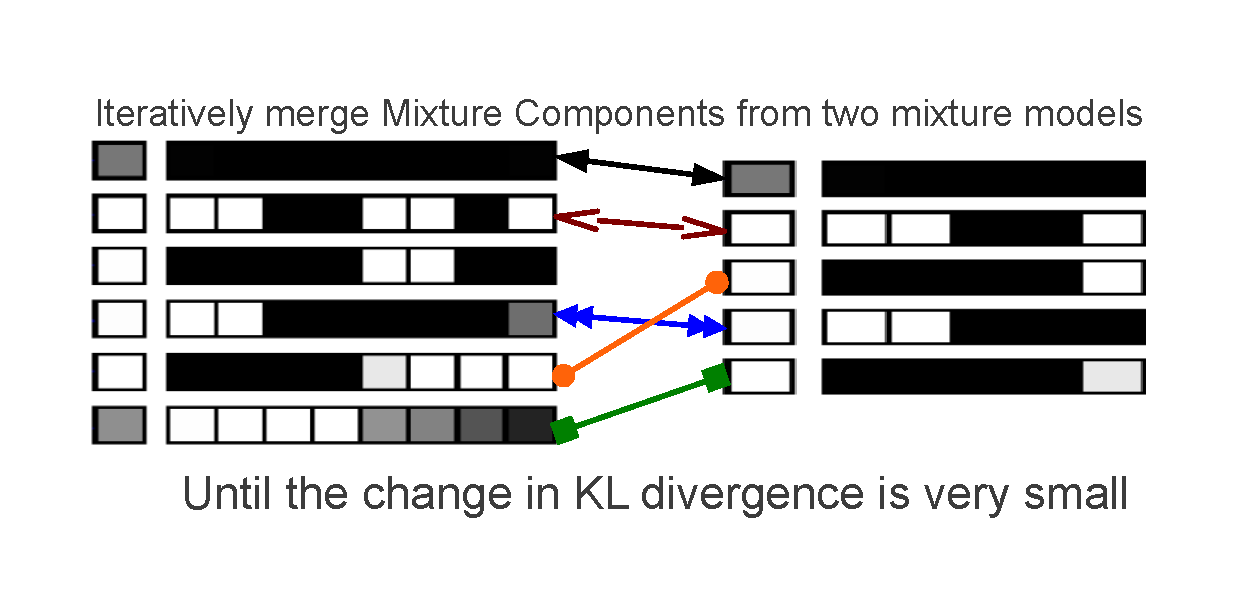
\includegraphics[trim=10mm 10mm 20mm 2mm,width=0.99\textwidth]{figures/idasecondpage}
\caption[Merging of Similar Mixture Components.]
{Simplified picture of multiresolution modelling using merging of mixture
components. We iteratively merge the similar components from different 
models until the change in KL divergence is very small. The different
arrow shapes show the pairwise similarity of mixture components.} 
\label{Fig:idasecondpage}
\end{figure}

We calculate the  pairwise KL divergence between 
all the components in two mixture models. We then  
select the similar components using minimum weight 
bipartite matching algorithm~\cite{west96graph} as shown in 
Figure~\ref{Fig:idasecondpage}. The similar components  are 
merged preserving the properties of component distributions 
and probability of random values in the mixture model. 
We iterate the matching shown in Figure~\ref{Fig:idasecondpage} 
and merging of mixture components until the  KL divergence is 
small enough. Finally, we retrain the mixture models in each 
resolution. Although mixture models are generated separately 
in each resolution, they incorporate information about the 
data in other resolutions.


\begin{figure}[h!]
\centering
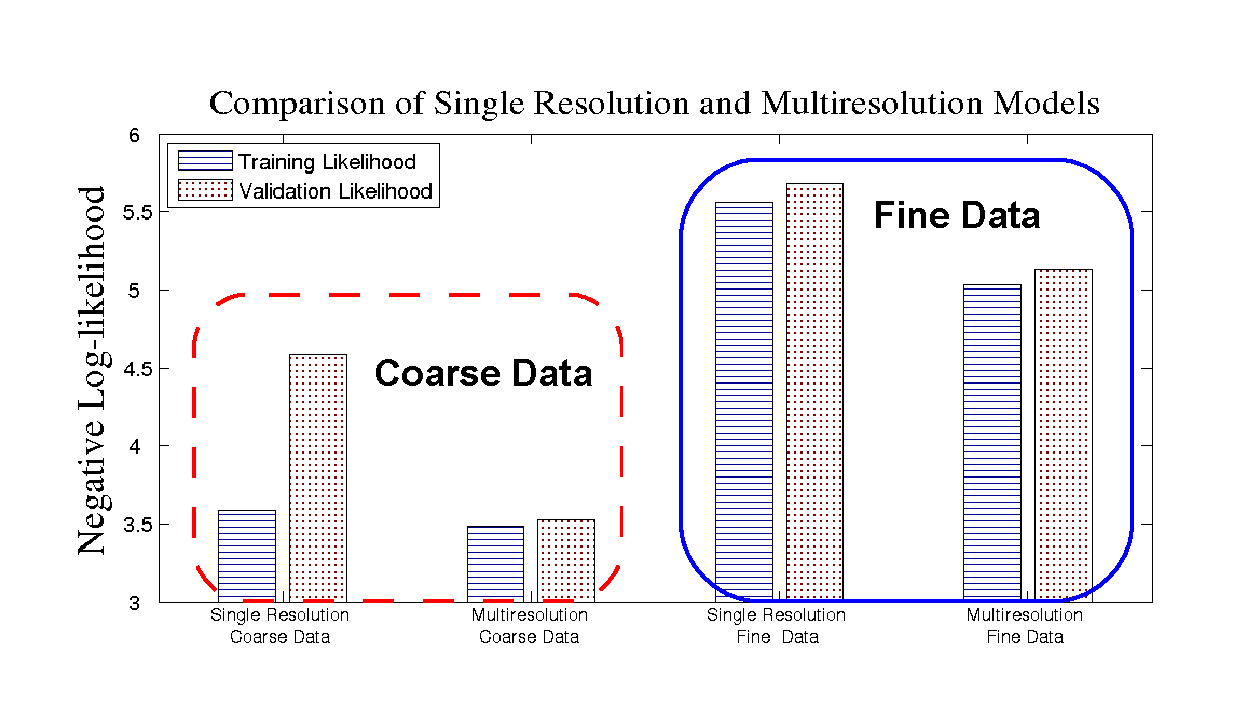
\includegraphics[trim=10mm 10mm 10mm 2mm,width=0.99\textwidth]{figures/nbarlkhood}
\caption[Performance of Mixture Models in Coarse and Fine Resolution.]
{Likelihood of multiresolution mixture models trained by merging of mixture 
components and individually trained mixture models in single resolution. 
Since the units in Y--axis is the negative log--likelihood, the shorter the 
bar the better the result. The improvement gained by multiresolution mixture 
model in the fine resolution is greater than that gained in the coarse 
resolution. The figure is adapted from~\citepub{c2}.} 
\label{Fig:barlikelihood}
\end{figure}

The algorithm generates plausible results when the algorithm is 
experimented on multiresolution chromosomal amplification datasets 
discussed in Section~\ref{s:multchrdata}. The bar diagram in the 
Figure~\ref{Fig:barlikelihood} depicts the improvements gained by 
multiresolution models over single resolution models. The figure 
shows training and validation likelihood of the multiresolution 
and independent single resolution mixture models trained 
in a 10--fold cross--validation setting. Since the units in Y--axis 
is negative log--likelihood, the shorter the bar better the result. 
The Figure~\ref{Fig:barlikelihood} shows the two different conditions 
of the likelihood: first, the performance of single resolution, and 
the multiresolution model on the coarse data, which is enclosed in 
the dashed rectangle in the left side of the  Figure~\ref{Fig:barlikelihood}. 
Second, Figure~\ref{Fig:barlikelihood} 
also shows performance of the single resolution and the multiresolution 
models on the  fine data which is enclosed in solid rectangle in the 
right side of the figure.


Scrutinising the results inside both the dashed and the solid 
rectangles in the Figure~\ref{Fig:barlikelihood}, the performance 
of the multiresolution model is markedly better in  the coarse
resolution and slightly better in the fine resolution. The 
improvement in the performance of the multiresolution model in 
the coarse resolution is greater than that in the fine resolution. 
This is because the number of data samples is comparatively smaller 
in the coarse resolution to add more information to the model
in the fine resolution. The results also show that the models trained 
in the multiresolution setting generalises better on the future
unseen data. As discussed in Section~\ref{s:meringMixCompo},
the performance of the models are better in coarse resolution
because of the curse of dimensionality. We also performed the 
two--tailed t--test to ascertain the statistical significance 
of the result on the data likelihood~\cite{walpole2012}. 
The results also show that both the validation and the training 
likelihoods are statistically significant when the 
significance level, $\alpha$, is 0.1. 


\section[Multiresolution Mixture Components]
{Multiresolution Mixture Components from Domain Ontology}
\label{s:DomainOnto}

\begin{figure}[h!]
\centering
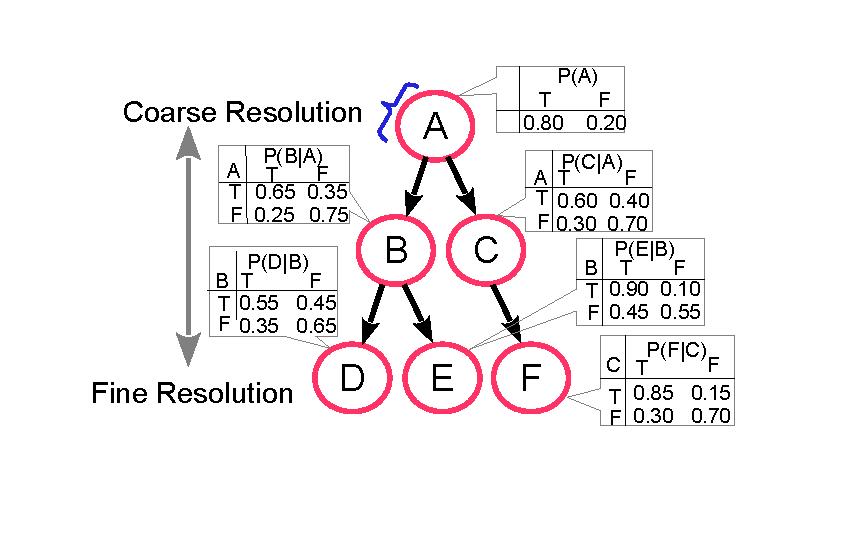
\includegraphics[trim=15mm 20mm 20mm 5mm,width=0.99\textwidth]{figures/bnnfig1}
\caption[Bayesian Network from Domain Knowledge.]
{A structure of the Bayesian network from the apriori domain 
knowledge shown in Figure~\ref{Fig:oncology}. The figure shows both
Bayesian Network with nodes and edges; and the associated conditional 
probability tables. The figure is adapted from~\citepub{c3}. } 
\label{Fig:oncobnn}
\end{figure}


Multiresolution data often forms hierarchical structure  as discussed
in Chapter~\ref{ch:analysismultires}. The domain ontology used in this 
thesis is known apriori from the application area. Consequently, we 
can exploit this structural information from the application area to 
determine the relationships between data resolutions. Therefore,
we can determine the structure of the Bayesian network as shown in the  
Figure~\ref{Fig:oncobnn} with some realistic assumptions for computational
efficiency. For this reason, we do not learn the structure of Bayesian 
networks in our contribution. The  assumptions are that the data features 
in the coarse resolution form the root and branches near the root of 
the Bayesian network. Similarly, the data features in the finer 
resolutions form the branches towards the  leaves and the leaves
of the Bayesian network. Additionally, we can assume that the  
directed arrows originate from the features in the coarse 
resolution. 

 
Figure~\ref{Fig:oncobnn} shows a Bayesian network generated 
from the hierarchical structure of data depicted in the 
Figure~\ref{Fig:oncology}. In the real world, although the hierarchical 
structure as shown in the Figure~\ref{Fig:oncology} are known, 
data in all the resolutions in the structure may not be available. 
Nevertheless, Bayesian networks have been known for their prowess 
in missing value imputation~\cite{dizio2004}. Therefore, in~\citepub{c3}, 
Bayesian networks in the component distributions are used to 
impute missing data resolutions. Experimental results in~\citepub{c3} 
show that Bayesian networks satisfactorily imputes missing data 
resolutions.

\begin{figure}[h!]
\centering
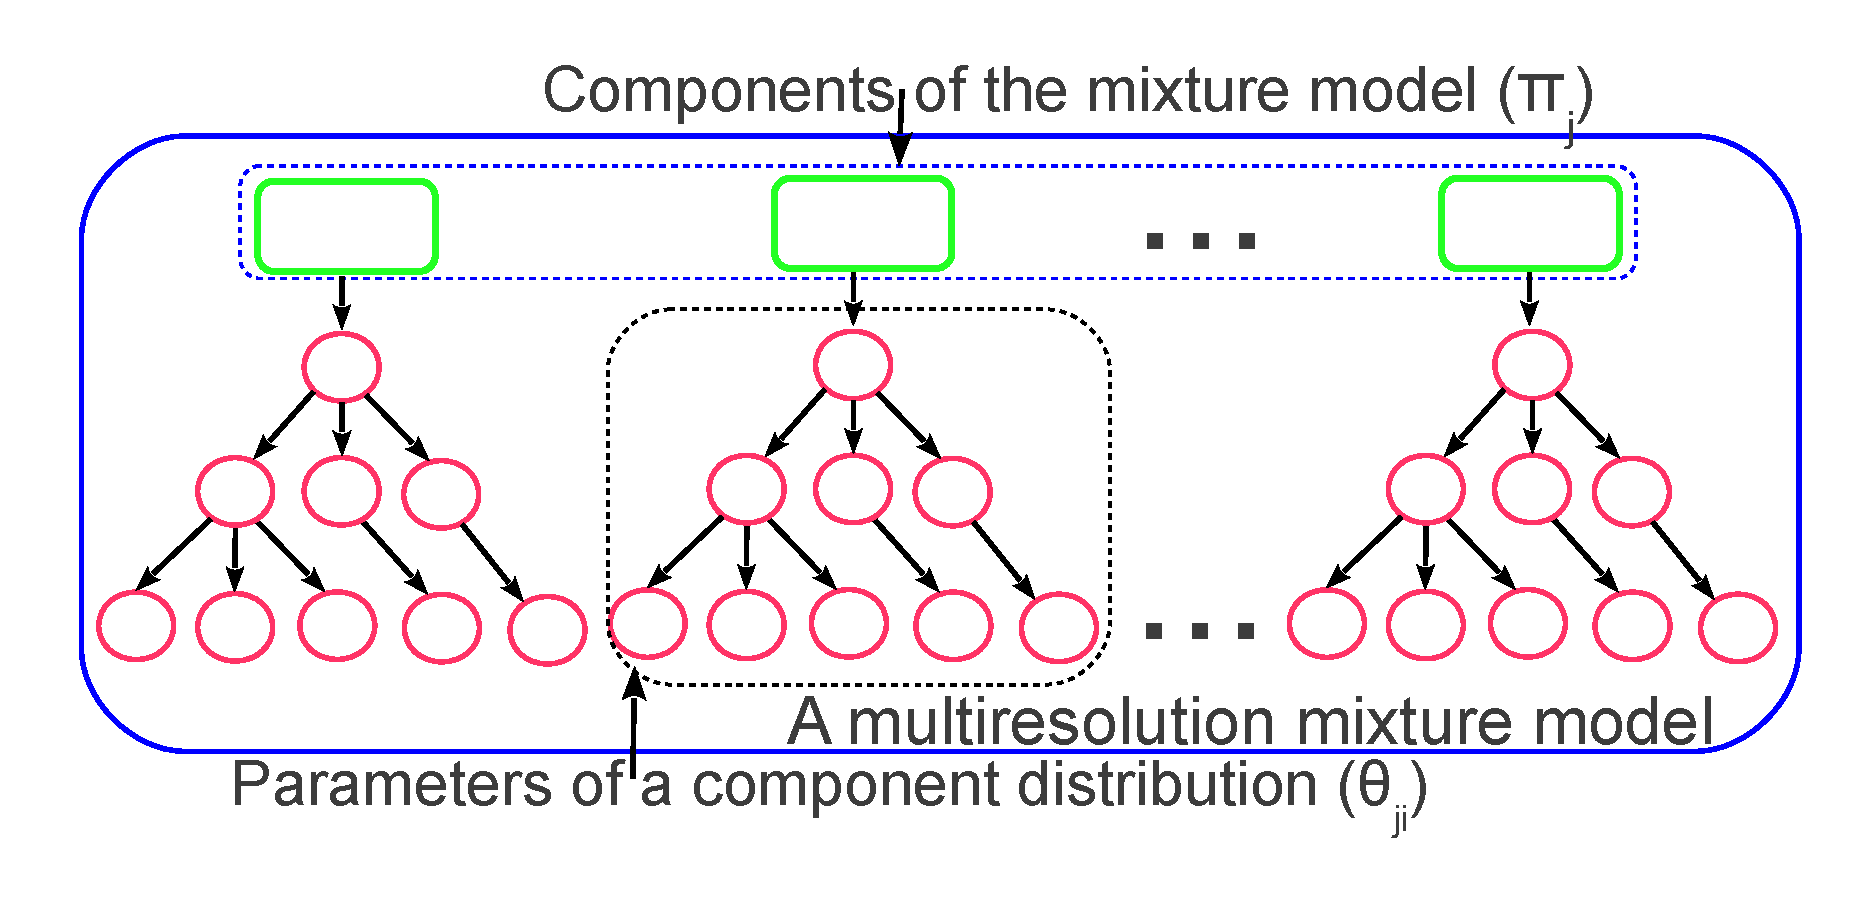
\includegraphics[trim=12mm 15mm 15mm 5mm,width=0.97\textwidth]{figures/multiresmix}
\caption[Multiresolution Mixture Model.]
{Structure of multiresolution mixture model whose components
are Bayesian networks. The figure is adapted from~\citepub{c3}.} 
\label{Fig:multiresmix}
\end{figure}

Figure~\ref{Fig:multiresmix} depicts the structure of the
proposed mixture model in~\citepub{c3} for data in multiple 
resolutions. The three solid rectangles on the top represent 
different mixture coefficients, $\pi$. Similarly, the three
network of nodes denote the three component distributions.
Each node defines a parameter of the component distributions, 
$\theta$. The structure of the component  distribution is 
determined from the domain knowledge. Since, the structure 
of Bayesian network is known, the  parameters of these 
Bayesian networks can be learned  in the maximum likelihood 
framework~\cite{barberBRML12}. If some of the data are missing,
we need some assumptions to learn the parameters of the 
Bayesian networks. One of such similar assumption is founded 
from the Potts model~\cite{baxter08,potts52} where we
estimate the CPD of the child (C) given parent (P) as:
$P(C \mid P)=0.9$.

After learning the Bayesian networks,  and imputing the missing
values, the next step is to learn the mixture models. First of 
the challenges confronting the learning of mixture model is the
model selection, i.e., determining the optimal number of 
component distributions~\cite{fraley1998}. Similarly, learning 
the parameters of the component distributions involves learning 
the parameters of those networks. In general framework for 
the EM algorithm, we can assign only a single probability value 
to a node in the mixture model~\cite{expectmax}. However, each 
variable in Bayesian network consists of minimum of two 
probability values denoting the CPD of the nodes. Hence, we 
learn the mixture  model in the two step procedure. First, we 
learn the the parameters of individual Bayesian networks in 
the framework of Bayesian networks~\cite{barberBRML12,heckerman1999}.
Second, we transform the networks to vectors to learn the 
parameters of mixture  model using the EM  algorithm as 
in~\cite{tikka2007b}.

\begin{figure}[h!]
\centering
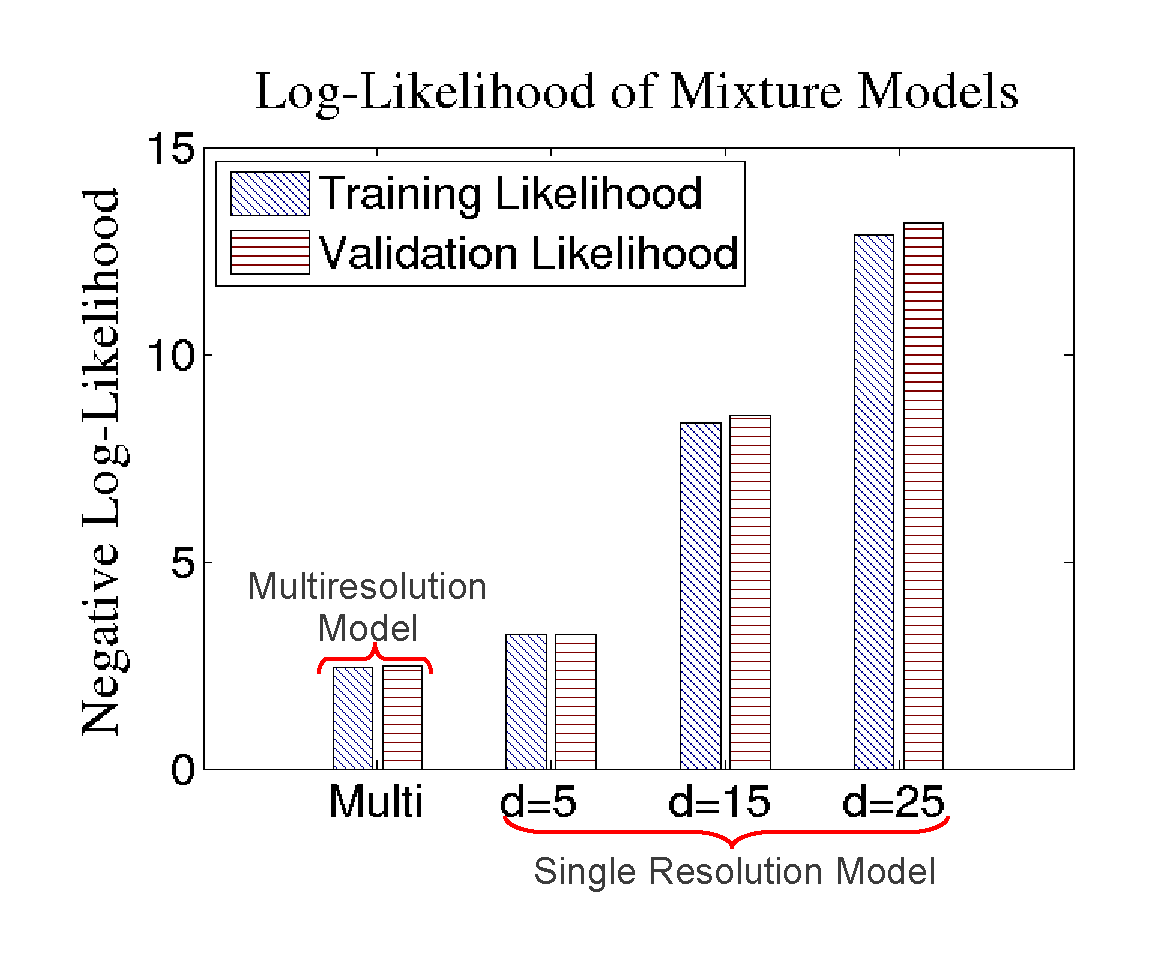
\includegraphics[trim=12mm 10mm 10mm 5mm,width=0.98\textwidth]{figures/barlkhood}
\caption[Comparison of Performance of the Mixture Models.]
{Likelihood of single resolution and multiresolution 
mixture model on simulated dataset. Since the units in 
Y--axis is the negative log--likelihood, shorter the bar 
better the result. The performance of multiresolution 
mixture models surpasses that of all the single resolution
models. Reprinted with permission from~\citepub{c3}.} 
\label{Fig:barmultires}
\end{figure}

In addition to the multiresolution chromosomal amplification 
datasets discussed in Section~\ref{s:multchrdata}, we 
have in~\citepub{c3} experimented with a simulated 
dataset that allows observation of complete data
without missing resolutions. 
The bar diagram in the Figure~\ref{Fig:barmultires} 
displays the performance of the multiresolution 
mixture model trained in a 10--fold cross--validation 
setting and also three different single resolution 
mixture models trained individually in each resolution. 
Since units used in the Y--axis is negative log--likelihood, 
the shorter the bar, better the result. The 
Figure~\ref{Fig:barmultires} shows two different conditions 
of likelihood: training  and validation. However,  
the results do not depict change in training 
and validation likelihood during model selection instead  
they  show the difference in training and validation 
likelihoods after the selection of components. 

The Figure~\ref{Fig:barmultires} shows that the performance
of the multiresolution mixture model  is markedly better than the 
three single resolution models. Log--likelihood is comparatively 
poor in dimensionality of 15, and 25 because 
of the larger data dimensionality demonstrating curse of
dimensionality. The likelihood of the 
proposed multiresolution model is better than the data with 
the smallest dimensionality of five in single resolution. The 
results show that proposed multiresolution mixture model 
produces plausible results in addition to providing single 
analysis solution for the data in multiple resolutions.


\section[Semantic Multiresolution Modelling]
{Multiresolution Semantic Subgroup Discovery}
\label{s:Semantic}

As discussed in Section~\ref{s:ontologymulti}, semantic data 
mining methods have been gaining popularity in the data mining
domain. Similarly, banded matrices have also found usage in 
data mining domain~\cite{elden2007,garriga2011banded}. In~\citepub{j2}, 
we comprehensively analyse multiresolution data using a three 
stage methodology depicted in Figure~\ref{Fig:sematicworkflow}. 
In the contribution, we explain the clustering generated by 
mixture models using semantic data mining methods, and visualise 
the clusters and the semantic rules using the banded matrices. 


\begin{figure}[h!]
\centering
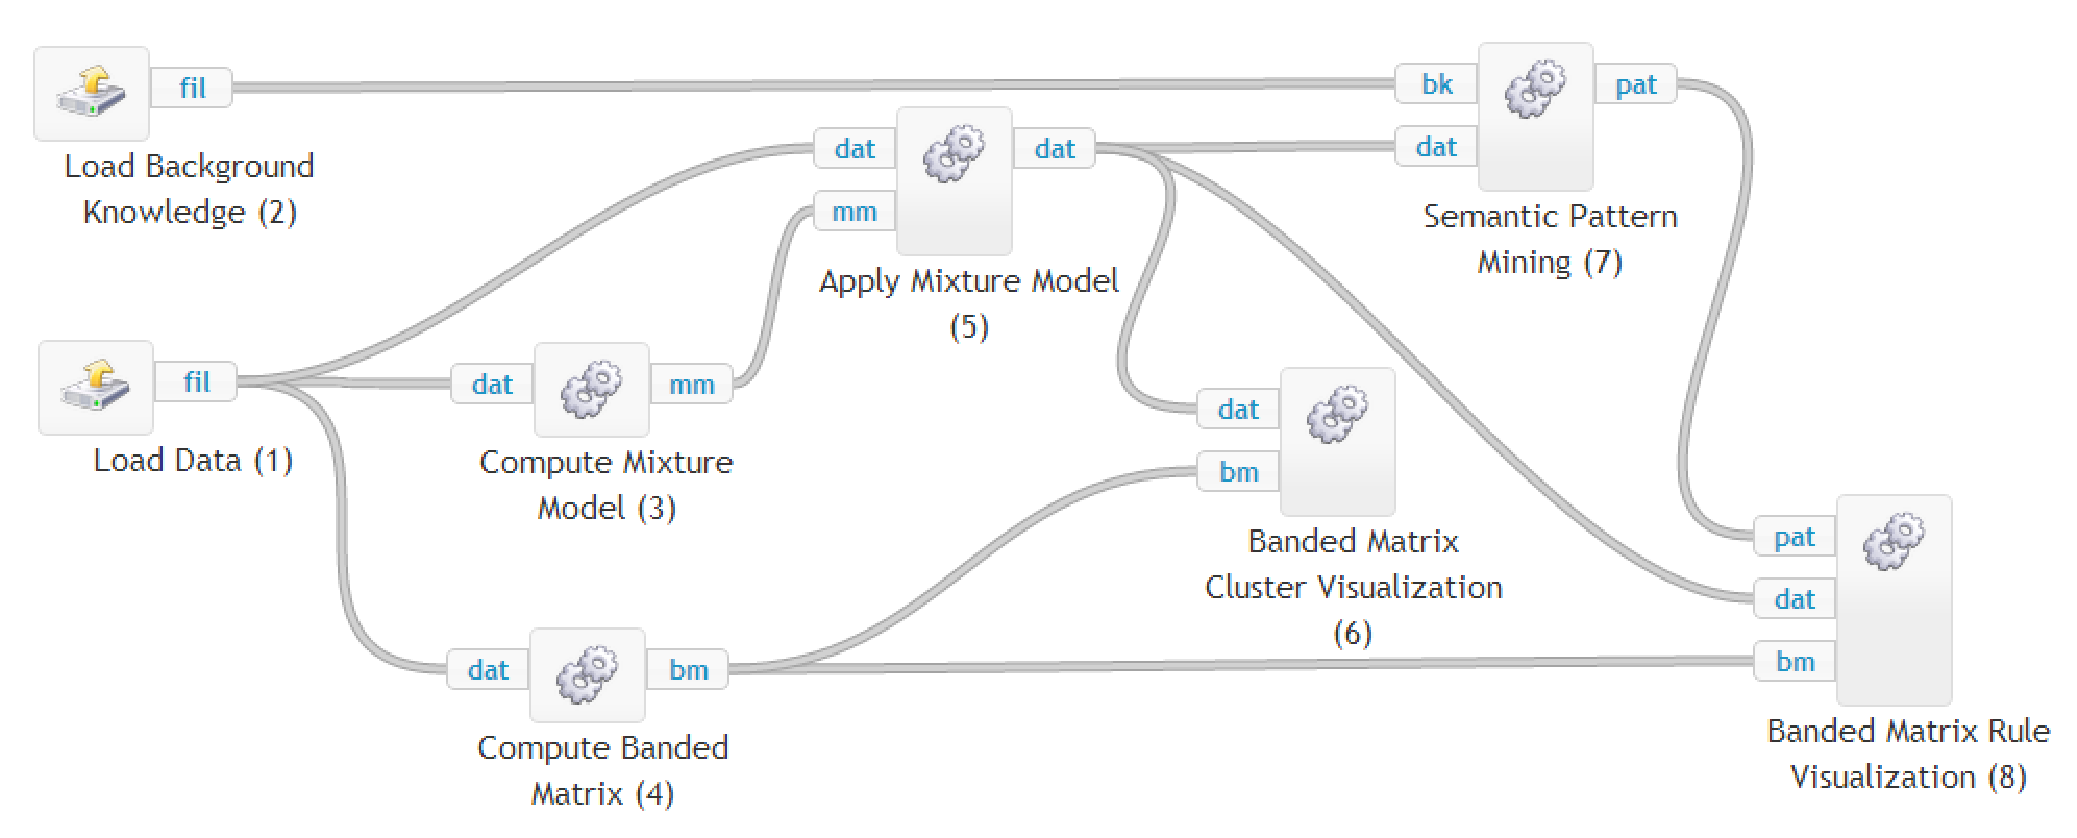
\includegraphics[trim=15mm 7mm 15mm 2mm,width=0.9\textwidth]{figures/sematicworkflow}
\caption[Workflow of Semantic Data Mining of Cluster.]
{The workflow for comprehensive analysis of multiresolution
data using a combination of probabilistic model based clustering, 
semantic data mining, and banded matrices. Reprinted with permission 
from~\citepub{j2}.} 
\label{Fig:sematicworkflow}
\end{figure}

Figure~\ref{Fig:sematicworkflow} depicts the working of the three
part methodology. The figure shows that input to the methodology 
is the empirical data and additional background knowledge. 
The additional background knowledge is used by the 
semantic data mining algorithm to supplement the analysis of the
empirical data. As cancer is a heterogeneous and multifactorial 
disease~\cite{king2002genetic}, we use additional background 
knowledge with an aim to better understand and
interpret the results. The additional knowledge 
provided to the semantic data mining algorithm comprises 
of fragile sites~\cite{durkin07,schwartz06}, cancer 
genes~\cite{futreal2004}, amplification hotspots~\cite{myllykangas06}, 
and virus integration sites~\cite{khoury2013,zurHausen2009}.
Finally, the taxonomies of hierarchical regions of chromosomes
discussed in Section~\ref{s:multchrdata} are also used as 
additional background knowledge so that semantic data mining
methods are able to analyse multiresolution data.

\begin{figure}[h!]
\centering
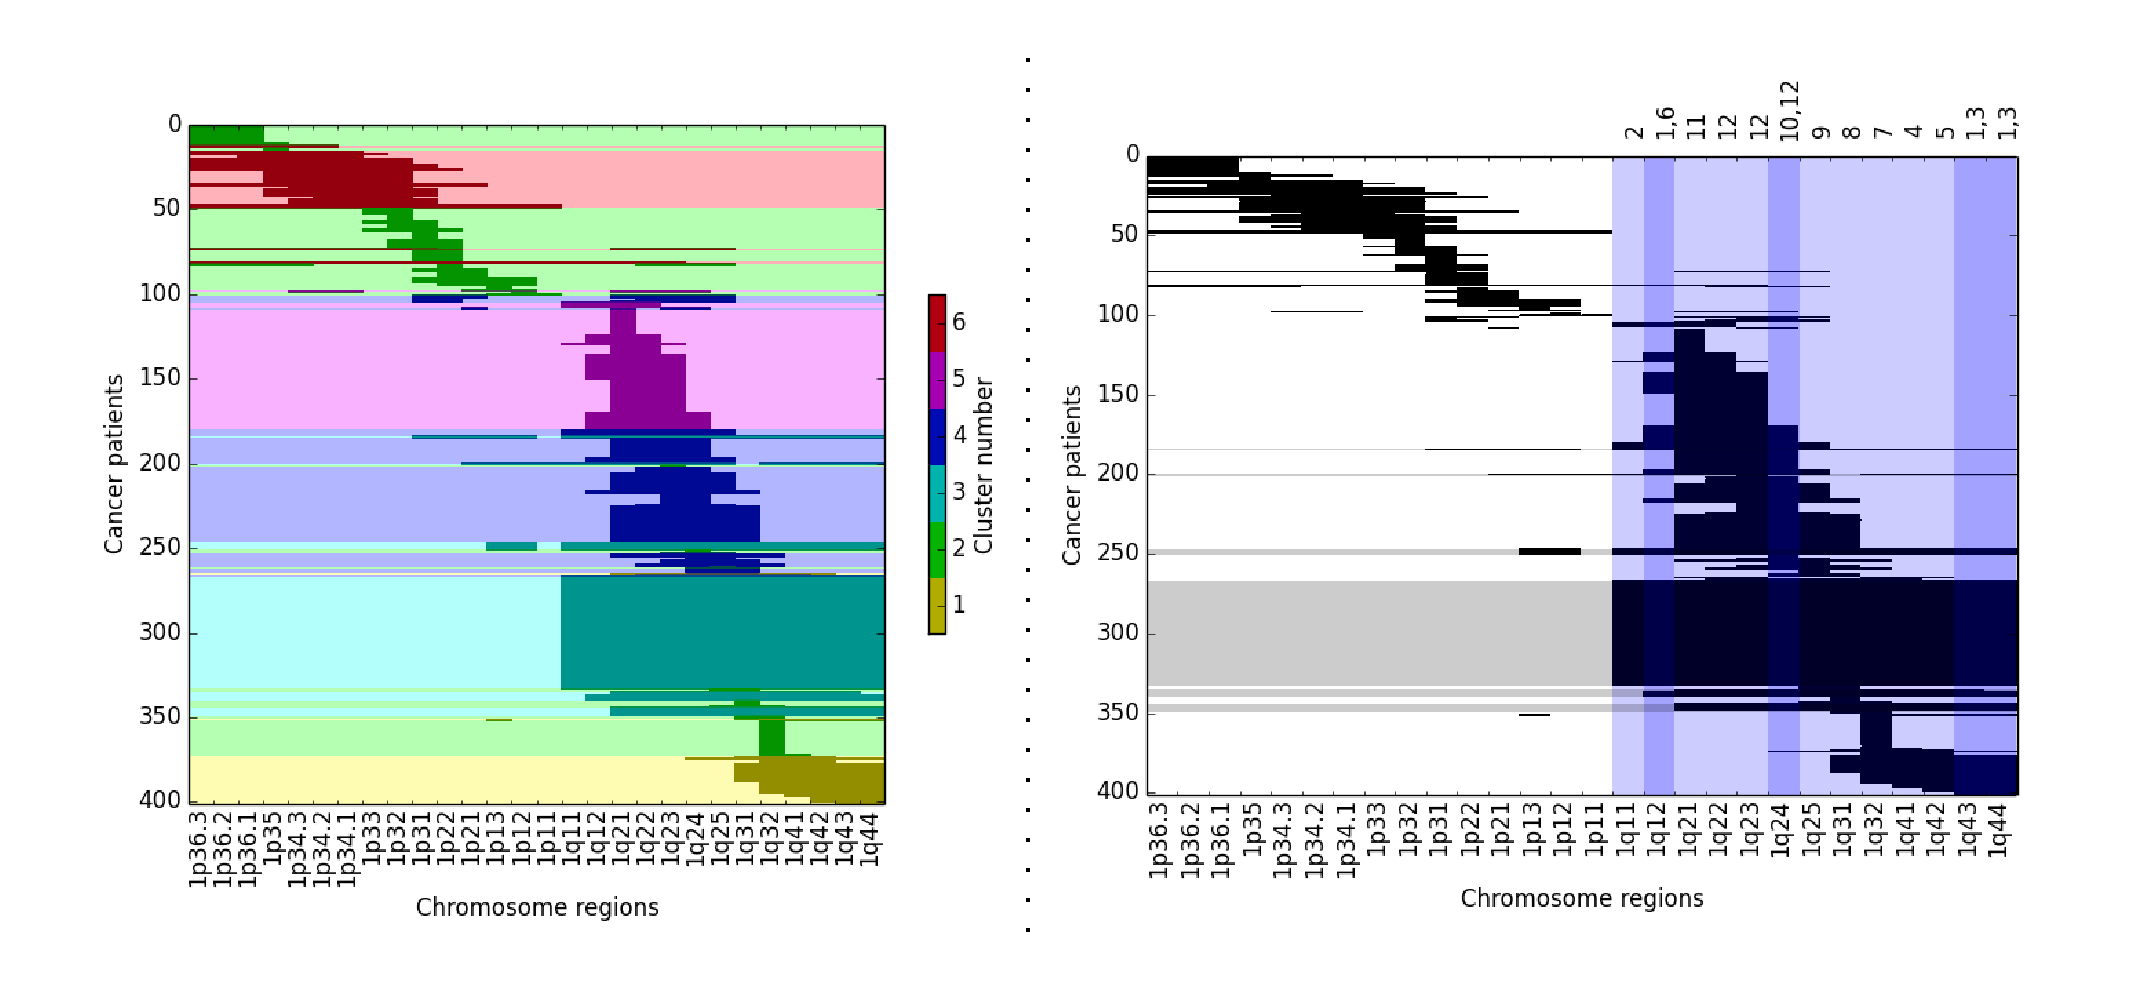
\includegraphics[trim=15mm 9mm 15mm 8mm,width=0.99\textwidth]{figures/clusterrules}
\caption[Visualisation of Clusters and Rules through Banded Matrices.]
{The comprehensive analysis of multiresolution data using
a combination of probabilistic model based clustering, 
semantic pattern mining, and banded matrices. Figure on 
the left panel depicts the clusters overlayed on the banded 
structure of data. Similarly, figure on the right panel depicts
the both clusters and semantic rules overlayed on the banded
structure of the data. For the clarity of presentation, the figure on
the right depicts only cluster 3 and the rules explaining only cluster 3.
Figures are adapted from~\citepub{j2}.} 
\label{Fig:clusterrules}
\end{figure}

Mixture models provide an ability to cluster the data
considering the components in the mixture model as 
a cluster~\cite{mclachlan1988mixture,melnykov2010finite}.
We train the mixture model in a ten--fold cross--validation 
setting taking parsimony into account~\cite{tikka2007b}. 
%We then select the components that generalizes 
%the best on the left--out data samples taking parsimony 
%into account~\cite{tikka2007b}.
The results produced by
mixture models are complex to explain to the application 
area specialist. Efforts have, however, been made in the
past to make the results
understandable to the domain experts~\cite{Hollmen2007a}. 
In~\citepub{j2}, we explain the clusters with the rules 
generated by semantic data mining algorithms and visualisation 
produced by banded matrices. The cluster labels generated using 
clustering from mixture model  are used as class labels in 
semantic pattern mining algorithm along with the additional 
background knowledge. We use general purpose semantic 
subgroup discovery system, Hedwig, to find a hypothesis 
(a predictive model or a set of descriptive patterns) 
in domain ontology terms, given the training data and 
the domain knowledge in the form of 
ontologies~\cite{Vavpetic13jiis}. Hedwig, for instance,
is  developed by the collaborators 
in Jo\v{z}ef Stefan Institute in Slovenia who
are the co--authors in~\citepub{j2}.

\begin{table}[bt]
\centering
\begin{tabular}{clccc}\hline
\textbf{\#} & \textbf{Rules for cluster 3} & \textbf{TP} & \textbf{FP} & \textbf{Precision}\\\hline
1 & \texttt{Cluster3(X) $\leftarrow$ 1q43-44(X) $\wedge$ 1q12(X)} & 81 & 0 & 1.00  \\
2 & \texttt{Cluster3(X) $\leftarrow$ 1q11(X)} & 78 & 9 & 0.90  \\
3 & \texttt{Cluster3(X) $\leftarrow$ 1q43-44(X)} & 88 & 26 & 0.77  \\
4 & \texttt{Cluster3(X) $\leftarrow$ 1q41(X)} & 88 & 28 & 0.76  \\
5 & \texttt{Cluster3(X) $\leftarrow$ 1q12(X)} & 81 & 43 & 0.65  \\
6 & \texttt{Cluster3(X) $\leftarrow$ 1q32(X)} & 88 & 52 & 0.63  \\
7 & \texttt{Cluster3(X) $\leftarrow$ 1q31(X)} & 87 & 54 & 0.62  \\
8 & \texttt{Cluster3(X) $\leftarrow$ 1q25(X)} & 88 & 64 & 0.58  \\
9 & \texttt{Cluster3(X) $\leftarrow$ 1q24(X)} & 88 & 97 & 0.48  \\
10 & \texttt{Cluster3(X) $\leftarrow$ 1q21(X)} & 88 & 134 & 0.40  \\
11 & \texttt{Cluster3(X) $\leftarrow$ 1q22--24(X)} & 88 & 149 & 0.37  \\
12 & \texttt{Cluster3(X) $\leftarrow$ HotspotSite(X)} & 88 & 222 & 0.28 \\
13 & \texttt{Cluster3(X) $\leftarrow$ CancerSite(X)} & 88 & 245 & 0.26 \\
14 & \texttt{Cluster3(X) $\leftarrow$ FragileSite(X)} & 88 & 259 & 0.25 \\
\hline
\end{tabular}
\caption{Rules induced for 3 using semantic data mining algorithm Hedwig.}
\label{Tab:clus3rules}
\end{table}


We use the constrained banded matrices~\cite{garriga2011banded} to 
visualise the data.
In chromosomal amplification data, the matrices are constrained because the columns denote 
the specific and unchangeable chromosome regions. We, therefore, 
shuffle only the rows, i.e., only the samples and not the columns.
We then overlay the cluster information along the rows of the banded 
matrix as shown in the left panel  of the 
Figure~\ref{Fig:clusterrules} showing clear distinction among 
different clusters. In addition, we overlay the rules generated 
using the semantic subgroup discovery method as shown in the 
right panel of the Figure~\ref{Fig:clusterrules}. 
The visualised rules are tabulated in Table~\ref{Tab:clus3rules}.
The numbers above the rules on top right corner denote the position 
of rules in the table. A darker hue means that specific region
in chromosome appears in more than one rule denoted by more than 
one position of the rules in the table. Overlaying all the
clusters and the rules for each of the clusters will clutter
multitude of information on a single figure compromising the 
understandability of the visualisation. Therefore, we first 
visualise all the clusters in the data overlaying it on a 
banded matrix as shown in the left panel of the 
Figure~\ref{Fig:clusterrules}. Second, we visualise
only a single cluster and the rules describing that cluster as 
shown in the right panel of the Figure~\ref{Fig:clusterrules}.



The left panel of the Figure~\ref{Fig:clusterrules} distinctly 
shows different clusters proving the credibility of
the clustering results. Similarly, the rules visualised in 
the right panel of the Figure~\ref{Fig:clusterrules} identify
the amplifications in chromosomal regions that are 
responsible for certain cluster (cluster 3) and consequently, specific 
groups of cancer as reported in~\cite{myllykangas08}. In addition,
the rules generated by semantic data mining algorithm provide
additional insights into the clustering solutions. For example,
from the left panel of the Figure~\ref{Fig:clusterrules} cluster
3 is denoted by the pronounced amplification in regions 1q11-q44. 
The rule: \framebox[1.1\width]{Rule 1: \texttt{Cluster3(X) 
$\leftarrow$ 1q43--44(X) $\wedge$ 1q12(X)}} characterises 
81 out of 88 data samples that are in cluster 3 showing that
amplifications in regions  1q43--44 and 1q12 characterises 
cluster 3 and related cancers with good coverage and precision. 
Results show that whole region of  1q11--44 need not be aberrated 
to discriminate that specific cluster of cancers. This provides 
insights into the data and improvements  in the understandability 
of the amplification to the domain experts.




%We are interested in 
%modeling 0-1 data so we consider the mixture model of multivariate
%bernoulli distributions. The standard formulation of finite mixture 
%models of bernoulli distributions is shown in the equation. We are 
%interested in modelling a probability distribution P(x) in terms of 
%J-component distributions parameterized by theta .. js. We then mix
%them together to form the probability distribution. Since our data 
%is 0-1 data, the probability distribution is multivariate bernoulli 
%as shown on the right side of the equation. 'J' indexes the components 
%and 'I' indexes the data dimension. These parameters, theta, tell the 
%probability that a random variable takes the value 0 or 1. Estimation 
%of the model can be performed easily using EM algorithm. This is a 
%text book stuff and have been there since 1970s so I will not touch 
%this. We have an open-source program package to learn mixture models 
%of multivariate bernoulli distributions. 
%components each resolution.
%gives additional 
%practical usefulness to mixture models. Among many 
%different uses of Bayesian networks, we 
%The figure 
%depicts a mixture model having the Bayesian networks as the 
%components for data in multiple resolutions. 
%\section{Section Heading}

%although the dimensionality 
%of the multi-resolution data is 9. 

%The Figure~\ref{Fig:barmultires} does not show the difference
%between training and validation likelihood u


%There is growing interest
%in multiresolution modelling because of the benefits of combining
%multiple data


%Recent addition to the field of pattern mining is rule based learning, 
%often referred to as association rule is a popular data mining  
%methodology to determine the interesting relations between variables 
%based on different various measures of 
%interestingness~\cite{hipp00,klemettinen94,piatetsky91b,agrawal94}. 

%Additionally, algorithms for determining 
%emerging patterns which are itemsets that significantly differs from one class 
%to the next~\cite{novak09,dong99}. 
%Bayesian networks 
%have been widely used in application areas such as medicine, computational 
%biology and bioinformatics~\cite{friedman2000}.
%The component distributions of the mixture 
%model are Bayesian networks. 

 
%The additional background knowledge
%aid the data mining algorithm to garner information from
%the data. 
%input to the methodology is 

%The data is the chromosomal amplification data
%discussed in Section~\ref{s:multchrdata}. 

%Nevertheless, among the three 
%methods the weighted downsampling method produces comparatively 
%different result than majority decision and OR--function downsampling 
%methods. 



%The proposed 
%methods transform data in different resolutions to a single resolution,
%and combine them.

%This thesis extensively uses 
%pattern mining methods to complement and evaluate the 
%multiresolution modelling algorithm. Furthermore, semantic 
%data mining methods are used to analyze the multiresolution 
%data in presence of other background knowledge 
%in~\citepub{j2}. 
%Hence, this chapter starts with a brief 
%summary of pattern mining.

%Data traformation methods are also called sampling deterministic and.

%We overlay cluster information along the rows of banded matrix which  